\section{Experiment} \label{sec:experment}


In this section, we demonstrate the performance of the proposed method.
%
We compared the performance of the following methods in terms of FPR and TPR:

$\bullet$ {\tt CAD-DA}: proposed method

$\bullet$ {\tt CAD-DA-oc}: proposed method with only the extra-conditioning described in \S \ref{subsec:conditional_data_space} (extension the ideas in \cite{lee2016exact, duy2021exact} to our proposed setting)

$\bullet$ {\tt Bonferroni}: the most popular multiple hypothesis testing approach

$\bullet$ {\tt Naive}: traditional statistical inference

$\bullet$ {\tt No Inference}: AD after DA without inference

%
We note that if a method cannot control the FPR under $\alpha$, it is \emph{invalid} and we do not need to consider its TPR.
%
A method has high TPR indicates that it has low FNR.
%
We set $\alpha = 0.05$.
%
We executed the code on Intel(R) Xeon(R) CPU E5-2687W v4 @ 3.00GHz.

\subsection{Numerical Experiments.}

\textbf{Univariate case.} We generated $\bm X^s$ and $\bm X^t$ with $\mu^s_i = 0$, $\veps^s_i \sim \NN(0, 1)$, for all $i \in [n_s]$, and $ \mu^t_j = 2, \veps^t_j \sim \NN(0, 1)$, for all $j \in [n_t]$.
%
We randomly selected $5$ data points in the target domain and made them to be abnormal by setting $\mu^t_j = \mu^t_j + \Delta$.
%
Regarding the FPR experiments, we set $n_s \in \{ 50, 100, 150, 200 \}$, $n_t = 25$, and $\Delta = 0$.
%
In regard to the TPR experiments, we set $n_s = 150$, $n_t = 25$, and $\Delta \in \{ 1, 2, 3, 4\} $. 
%
Each experiment was repeated 120 times.
%
The results are shown in Fig. \ref{fig:fpr_tpr_1d}.
%
In the plot on the left, the {\tt CAD-DA}, {\tt CAD-DA-oc} and {\tt Bonferroni} controlled the FPR under $\alpha$ whereas the {\tt Naive} and {\tt No Inference} \emph{could not}. 
%
Because the {\tt Naive} and {\tt No Inference} failed to control the FPR, we no longer considered the TPR .
%
In the plot on the left, we can see that the {\tt CAD-DA} has highest TPR compared to other methods in all the cases, i.e., the {\tt CAD-DA} has lowest FNR compared to the competitors.



\begin{figure}[!t]
     \centering
     \begin{subfigure}[b]{0.492\linewidth}
         \centering
         \includegraphics[width=\textwidth]{fpr_1D}
         \caption{FPR}
     \end{subfigure}
     \hfill
     \begin{subfigure}[b]{0.492\linewidth}
         \centering
         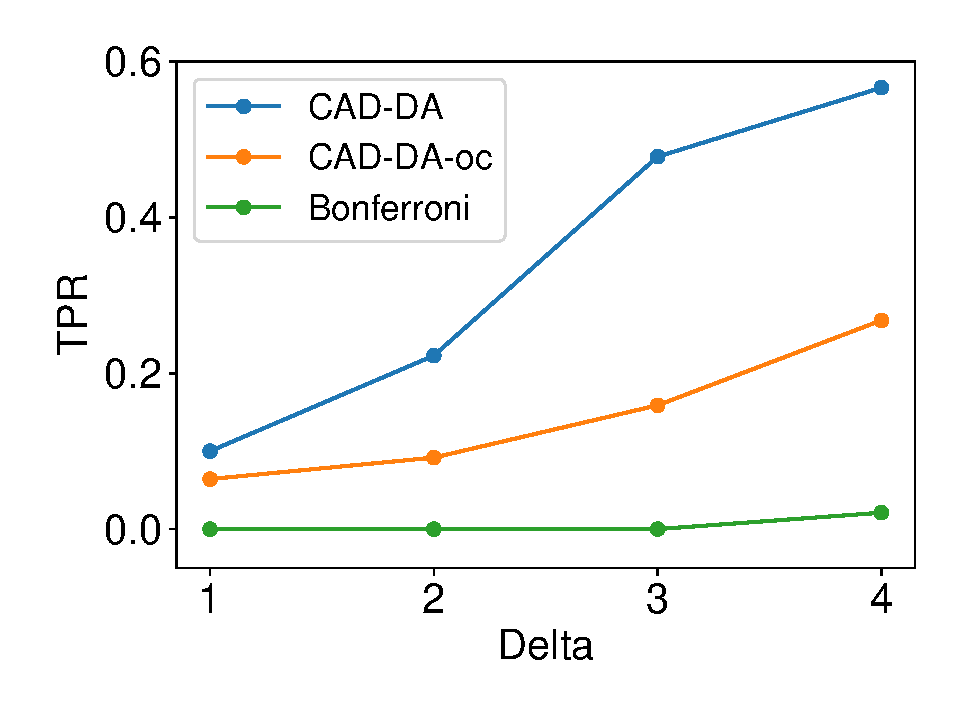
\includegraphics[width=\textwidth]{tpr_1D}
         \caption{TPR}
     \end{subfigure}
     \caption{FPR and TPR in univariate case}
     \label{fig:fpr_tpr_1d}
     
\end{figure}

\begin{figure}[!t]
     \centering
     \begin{subfigure}[b]{0.492\linewidth}
         \centering
         \includegraphics[width=\textwidth]{fpr_10D}
         \caption{FPR}
     \end{subfigure}
     \hfill
     \begin{subfigure}[b]{0.492\linewidth}
         \centering
         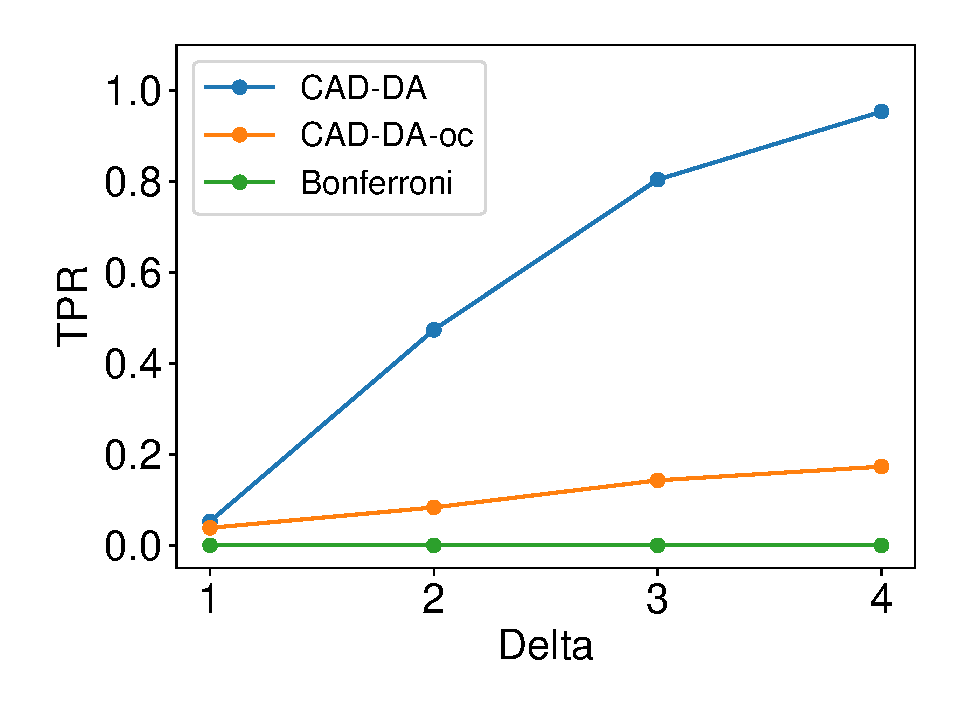
\includegraphics[width=\textwidth]{tpr_10D}
         \caption{TPR}
     \end{subfigure}
     \caption{FPR and TPR in multi-dimensional case}
     \label{fig:fpr_tpr_10d}
     \vspace{-8pt}
\end{figure}


\textbf{Multi-dimensional case.} We generated $X^s$ and $X^t$ with $X^s_{i, :} \sim \NN(\bm 0_d, I_d), \forall i \in [n_s]$, $X^t_{j, :} \sim \NN(\bm 2_d, I_d), \forall j \in [n_t]$, and the dimension $d = 10$.
%
The settings %for FPR and TPR experiments 
were the same as univariate case.
%
The results are shown in Fig. \ref{fig:fpr_tpr_10d}.
%
%The interpretation of the results is similar and consistent with the univariate case.
%
The important point we would like to note is that the difference in TPR between the {\tt CAD-DA} and {\tt CAD-DA-oc} in the multi-dimensional case is larger than that in the univariate case.
%
This indicates that the issue of extra-conditioning is more serious when increasing $d$.
%
If we naively extend the ideas in \cite{lee2016exact, duy2021exact} to our setting, the TPR will be low, i.e., the FNR is high.
%
In contrast, by introducing the hierarchical linear search step to remove the extra-conditioning, the FNR is significantly decreased by the proposed {\tt CAD-DA} method.


\textbf{Correlated data.} In this setting, we consider the case where the data is not independent.
%
We generated $X^s$ and $X^t$ with $X^s_{i, :} \sim \NN(\bm 0_d, \Xi), \forall i \in [n_s]$, $X^t_{j, :} \sim \NN(\bm 2_d, \Xi), \forall j \in [n_t]$, the matrix %$\Xi$ is defined as
%
$
\Xi = \left [\rho^{|i - j|} \right ]_{ij}, \forall i,j \in [d],
$
$\rho = 0.5$, and $d = 10$.
%
The settings for FPR and TPR experiments were also the same as univariate case.
%
The results are shown in Fig. \ref{fig:fpr_tpr_correlated}.
%
Additionally, we also conducted FPR and TPR experiments when changing $\rho \in \{ 0.2, 0.4, 0.6, 0.8\}$. We set $n_s = 150, n_t = 25$, $\Delta = 0$ for FPR experiments, and $\Delta = 4$ for the TPR experiments.
%
The results are shown in Fig. \ref{fig:fpr_tpr_correlated_change_rho}.
%
In essence,  the correlated data contains redundant information. 
%
This means that the effective sample size is smaller than the actual sample size. 
%
A smaller effective sample size reduces the amount of information available for the statistical test, making it less powerful. 
%
Therefore, the TPR tends to decrease when increasing the value of $\rho$.
%
However, in all the case, the proposed {\tt CAD-DA} method consistently achieves the highest TPR while controlling the FPR.

\begin{figure}[!t]
     \centering
     \begin{subfigure}[b]{0.492\linewidth}
         \centering
         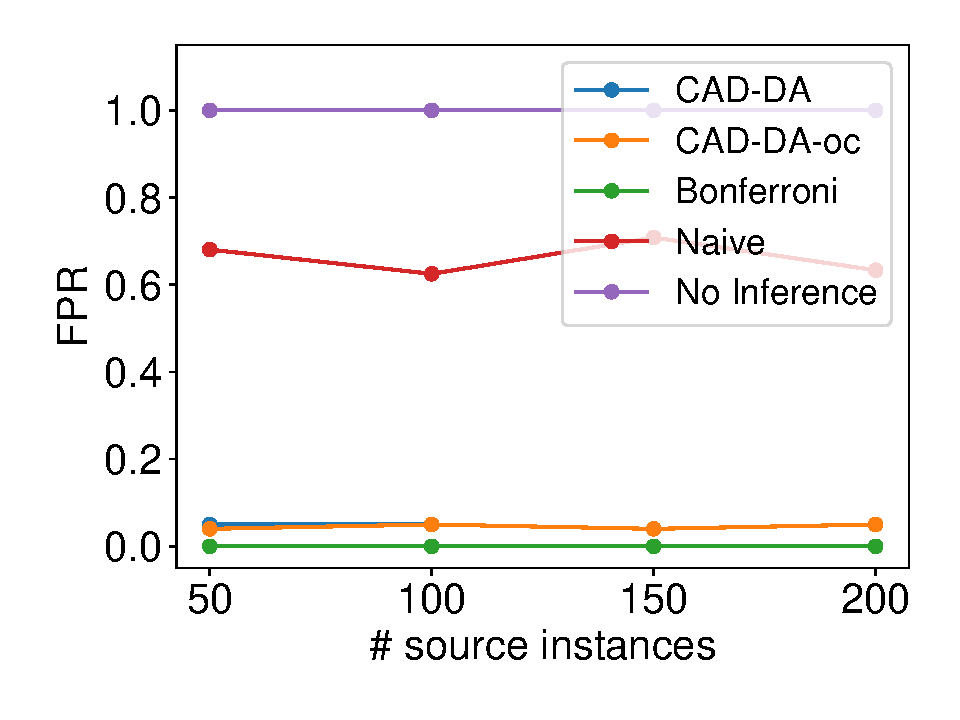
\includegraphics[width=\textwidth]{fpr_time_series}
         \caption{FPR}
     \end{subfigure}
     \hfill
     \begin{subfigure}[b]{0.492\linewidth}
         \centering
         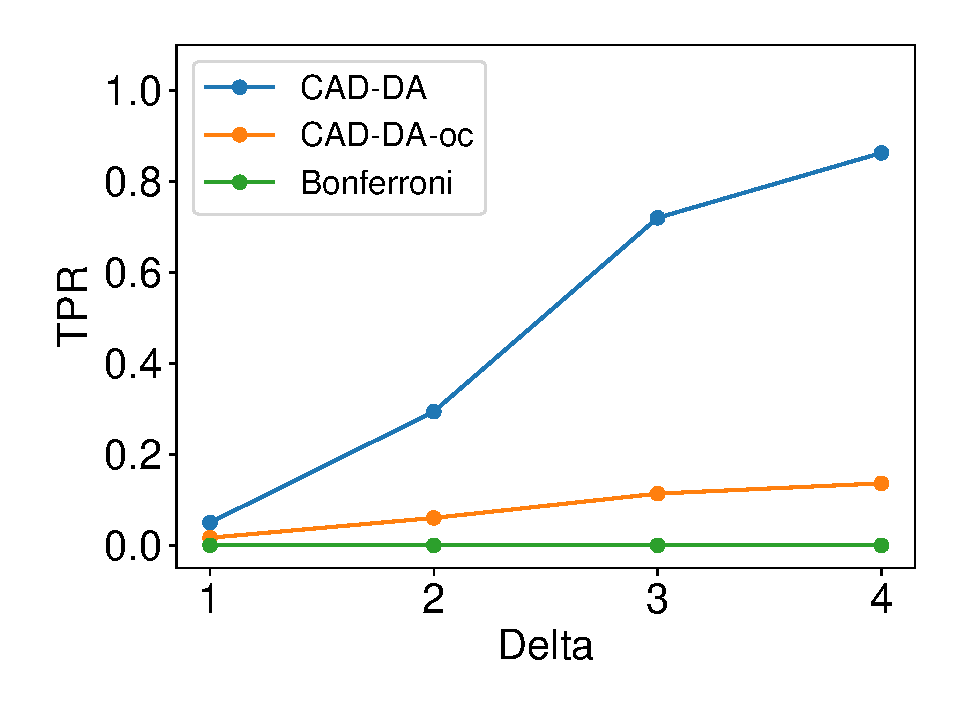
\includegraphics[width=\textwidth]{tpr_time_series}
         \caption{FPR}
     \end{subfigure}
     \caption{FPR and TPR in the case of correlated data}
     \label{fig:fpr_tpr_correlated}
\end{figure}

\begin{figure}[!t]
     \centering
     \begin{subfigure}[b]{0.492\linewidth}
         \centering
         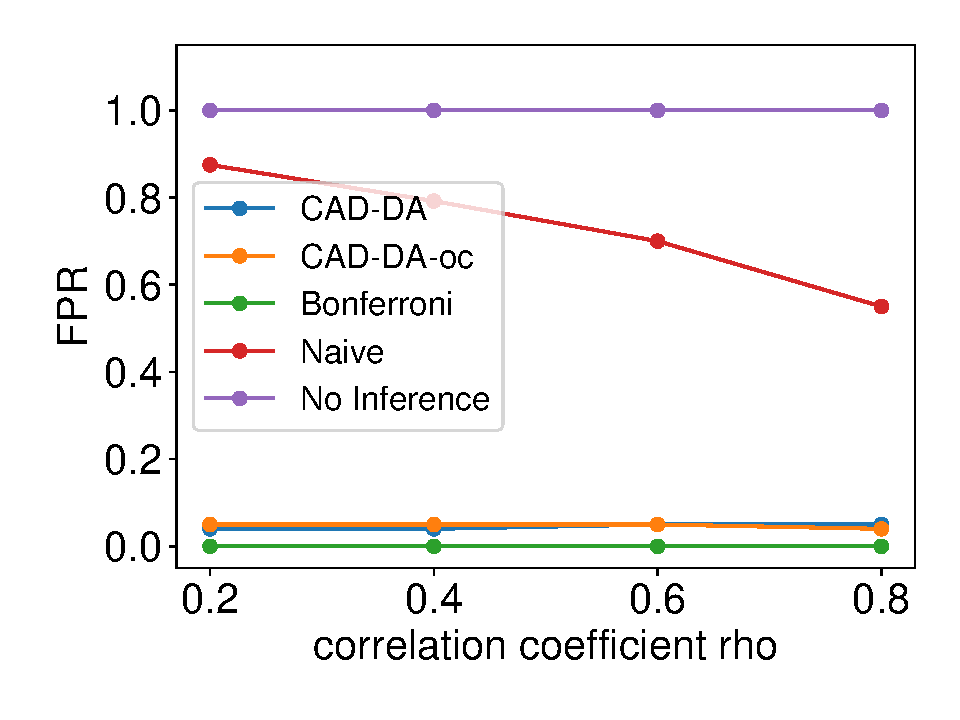
\includegraphics[width=\textwidth]{fpr_change_rho}
         \caption{FPR}
     \end{subfigure}
     \hfill
     \begin{subfigure}[b]{0.492\linewidth}
         \centering
         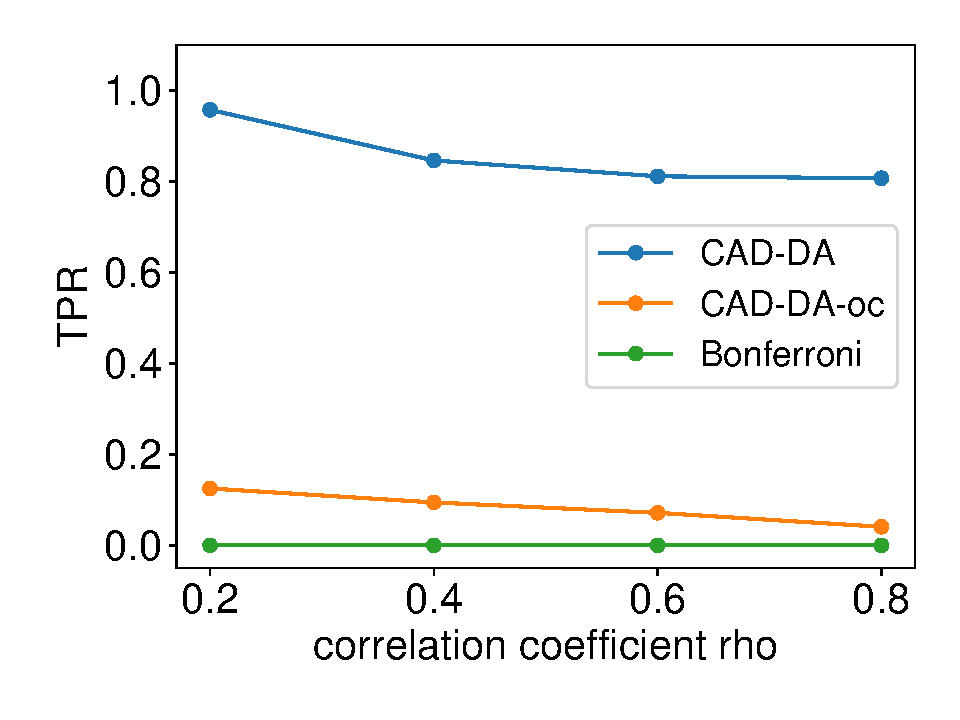
\includegraphics[width=\textwidth]{tpr_change_rho}
         \caption{TPR}
     \end{subfigure}
     \caption{FPR and TPR when changing  $\rho$}
     \label{fig:fpr_tpr_correlated_change_rho}
\end{figure}


\textbf{Comparison with \cite{tsukurimichi2022conditional} and robustness experiments.}
%
Since the method of \cite{tsukurimichi2022conditional} is not applicable to our proposed setting, we have to introduce an extended setting for conducting the experiments of FPR comparison with their method.
%
The details are provided in Appendix \ref{appx:comparison_with_tsukurimichi}.
%
The results are shown in Fig. \ref{fig:comparison_with_tsukurimichi}.
%
The proposed {\tt CAD-DA} could properly control the FPR under $\alpha = 0.05$ whereas the existing method \cite{tsukurimichi2022conditional} failed because it could not account for the influence of DA process.
%
Additionally, we conducted the experiments on the robustness of the {\tt CAD-DA} when the noise follows Laplace distribution, skew normal distribution, $t_{\rm 20}$ distribution, and variance is estimated from the data. 
%
The details are shown in Appendix \ref{appx:robustness}.
%
Overall, the {\tt CAD-DA} method still maintained good performance.

\vspace{-4pt}

\subsection{Real-data Experiments}

\vspace{-2pt}

We performed power comparison on real-data.
%
We used the \emph{NeuroKit2} simulator \cite{Makowski2021neurokit} to generate realistic respiration signals ($n_s = 150$) used for source dataset, and heart-beat signals ($n_t = 25$) used for target dataset, each with a dimensionality of $d = 12$.
%
We repeated the experiment $N \in \{ 120, 240\} $ times.
%
The results are shown in Tab. \ref{tbl:real_data_1}.
%
While the {\tt Bonferroni}, {\tt CAD-DA-oc} and {\tt CAD-DA} could control the FPR, the {\tt CAD-DA} had the highest TPR in all the cases.
%
We note that, in the case of Bonferroni correction, the TPRs were all 0.0 which indicates that this method is too conservative and all the true anomalies were missed out even though there exists, i.e., FNR = 1.0.


\begin{figure}[!t]
\begin{minipage}{0.48\linewidth}
  \centering
  % include first image
  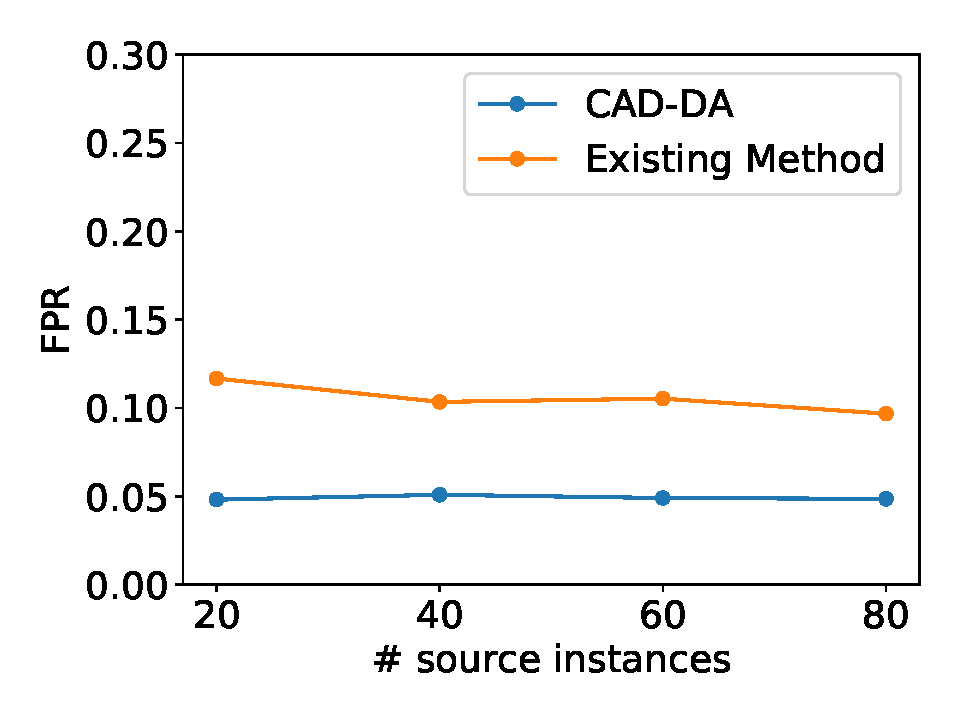
\includegraphics[width=\linewidth]{comparison_with_tsukurimichi}  
\caption{FPR comparison with \cite{tsukurimichi2022conditional}}
\label{fig:comparison_with_tsukurimichi}
\end{minipage}
\hspace{0.5mm}
\begin{minipage}{0.48\linewidth}
  \centering
  % include first image
  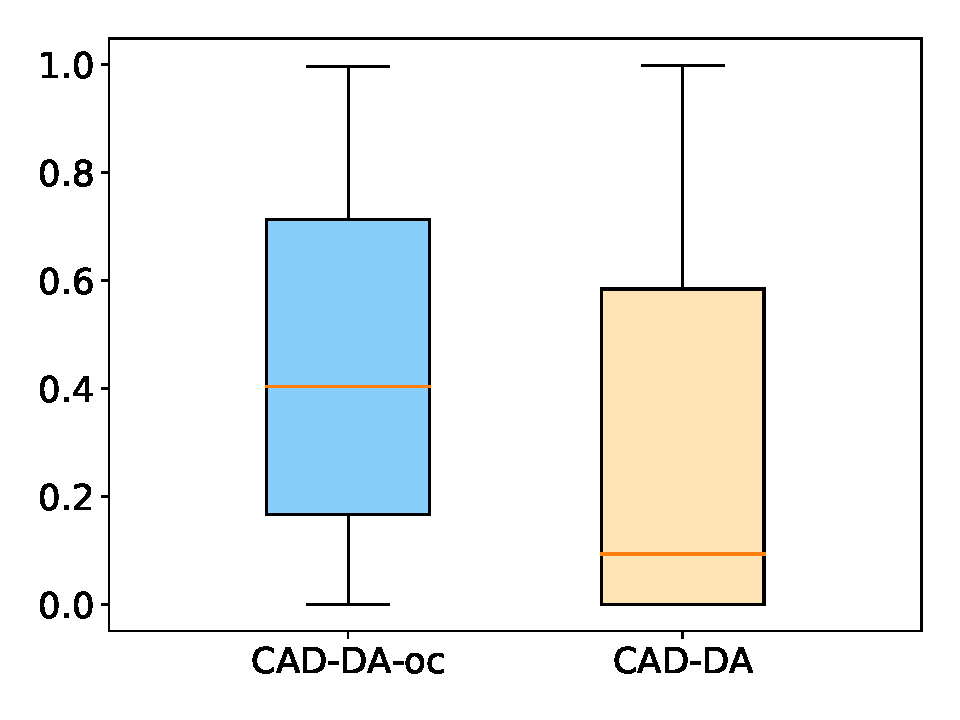
\includegraphics[width=\linewidth]{boxplot}  
\caption{Boxplots of $p$-values}
\label{fig:boxplot}
\end{minipage}
\end{figure}


\begin{table} [!t]
\renewcommand{\arraystretch}{1.1}
\centering
\caption{Comparison on real-data.}
%\vspace{-2pt}
\begin{tabular}{ |l|c|c|c|c| } 
  \hline
  & \multicolumn{2}{|c|}{$N = 120$} & \multicolumn{2}{|c|}{$N = 240$} \\ 
  \hline
  & ~ FPR ~&~TPR~&~FPR~&~TPR~\\
  \hline
   \hline
 \textbf{No Inference} & 1.00 & N/A & 1.00 & N/A \\ 
  \hline
 \textbf{Naive} & 0.90 & N/A & 0.90 & N/A \\ 
 \hline
 \textbf{Bonferroni} & \textbf{0.00} & 0.00 & \textbf{0.00} &  0.00 \\ 
  \hline
 \textbf{CAD-DA-oc} & \textbf{0.05} & 0.12 & \textbf{0.04} & 0.07 \\ 
  \hline
 \textbf{CAD-DA} & \textbf{0.04} & \textbf{0.71} & \textbf{0.04} & \textbf{0.73}\\ 
 \hline
\end{tabular}
\label{tbl:real_data_1}
\vspace{-10pt}
\end{table}



Additionally, we compared the $p$-values of the {\tt CAD-DA-oc} and {\tt CAD-DA} on Heart Disease dataset, which is available at the UCI Machine Learning Repository.
%
We randomly selected $n_s = 150$ patients whose gender is male (source domain), $n_t = 25$ patients whose gender is female (target), and conducted the experiment to compute the $p$-value.
%
The experiments was repeated 120 times. The boxplots of the distribution of the $p$-values are illustrated in Fig. \ref{fig:boxplot}.
%
The $p$-values of the {\tt CAD-DA} tend to be smaller than those of {\tt CAD-DA-oc}, which indicates that the proposed {\tt CAD-DA} method has higher power than the {\tt CAD-DA-oc}.


%\begin{figure}[!t]
%  \centering
%  % include first image
%  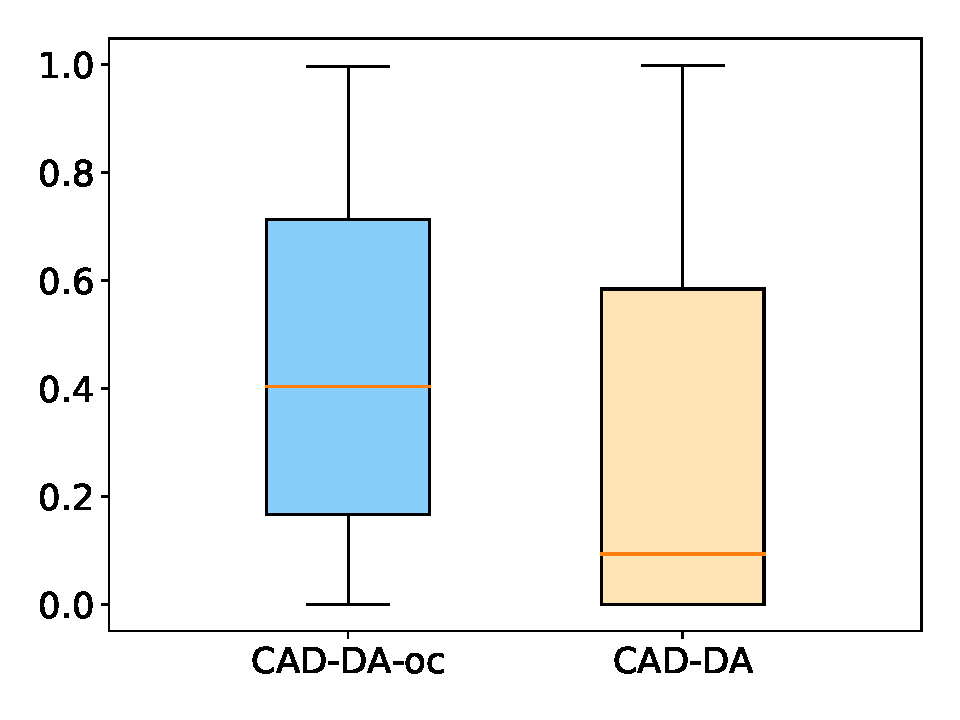
\includegraphics[width=.8\linewidth]{boxplot}  
%\caption{Boxplots of $p$-values}
%\label{fig:boxplot}
%\end{figure}





